\chapter{Why Mesoscopic Theory?}
\label{ch:why-mesoscopic-theory}

\textit{Mesoscopic theory keeps the population variables that clustered spiking networks actually use: how active each cluster is, how noisy that activity is at finite size, and how recurrent coupling moves the system between collective states. It is less detailed than a microscopic simulation, but more mechanistic than a phenomenological rate model.}

% ============================================================
\section{Microscopic models: accurate but high-dimensional}
\label{sec:microscopic-models-high-dimensional}
% ============================================================

A microscopic spiking model describes every neuron separately. For neuron $i$, one tracks a membrane variable, spike times, synaptic currents, and sometimes adaptation or conductance variables. The network state is therefore large: if there are $N$ neurons and several state variables per neuron, the phase space has dimension proportional to $N$.

A useful abstract form is
%
\begin{equation}
  X_i(t)=\sum_k \delta(t-t_i^k),
  \qquad
  \lambda_i(t)=\phi_i\!\left(h_i(t),\,\mathcal{H}_i(t)\right),
  \label{eq:microscopic-point-process}
\end{equation}
%
where $X_i(t)$ is the spike train of neuron $i$, $t_i^k$ are its spike times, $\lambda_i(t)$ is its conditional firing intensity, $h_i(t)$ is its current synaptic drive, and $\mathcal{H}_i(t)$ denotes spike-history variables such as refractoriness or adaptation. The function $\phi_i$ maps biophysical state to instantaneous spike probability.

For a current-based network, the drive can be written schematically as
%
\begin{equation}
  h_i(t)
  =
  I_i^{\mathrm{ext}}(t)
  + \sum_{j=1}^N J_{ij}\,(\kappa_{ij} * X_j)(t),
  \label{eq:microscopic-synaptic-drive}
\end{equation}
%
where $I_i^{\mathrm{ext}}$ is external input, $J_{ij}$ is the synaptic weight from neuron $j$ to neuron $i$, $\kappa_{ij}$ is a synaptic filter, and $*$ denotes convolution. The term $(\kappa_{ij} * X_j)(t)$ converts presynaptic spikes into postsynaptic current.

This model is faithful to the mechanism: spikes cause filtered synaptic events; synaptic events move membrane variables; membrane variables control future spikes. But for clustered networks the object of interest is not usually neuron $17$ or neuron $3012$. The scientific question is whether clusters enter and leave up-states, how long those states persist, and how stimulus input changes the collective state space.

The microscopic model is therefore the ground truth, not always the best explanatory coordinate system. It tells us what happened. A theory should tell us why the same kind of collective event would happen again when cluster size, coupling strength, or stimulus drive changes.

% ============================================================
\section{Macroscopic rate models: simple but often phenomenological}
\label{sec:macroscopic-rate-models-simple}
% ============================================================

A macroscopic rate model compresses the network to a small number of variables. In the simplest two-population excitation--inhibition model, the state is $(r_E,r_I)$, where $r_E$ and $r_I$ are population firing rates. A typical equation is
%
\begin{equation}
  \tau_\alpha \dot r_\alpha
  =
  -r_\alpha
  +
  \Phi_\alpha\!\left(
    \sum_{\beta\in\{E,I\}} W_{\alpha\beta} r_\beta
    + I_\alpha(t)
  \right),
  \qquad \alpha\in\{E,I\}.
  \label{eq:macroscopic-rate-model}
\end{equation}
%
Here $\tau_\alpha$ is a population time constant, $\Phi_\alpha$ is a static input--output function, $W_{\alpha\beta}$ is the effective coupling from population $\beta$ to population $\alpha$, and $I_\alpha$ is external drive.

This description is useful because it exposes fixed points, stability, gain, and bifurcations. If the effective recurrent excitation is strong enough, the equation can have a low-rate fixed point and a high-rate fixed point. That is the dynamical-systems skeleton of an up-state.

The limitation is that the variables are often phenomenological. The model may not say how $W_{\alpha\beta}$ depends on synaptic weights, how $\Phi_\alpha$ depends on spiking dynamics, or how intrinsic noise scales with the number of neurons. In clustered spiking networks this matters: metastable switching is not a small decorative correction. It is part of the phenomenon.

A deterministic rate equation with a manually added noise term can mimic switching, but it may not distinguish two mechanisms:
%
\begin{enumerate}[leftmargin=*]
  \item switching caused by finite population size in an otherwise multistable system;
  \item switching caused by deterministic high-dimensional dynamics such as mesoscopic chaos.
\end{enumerate}
%
The rotation question lives exactly at this boundary.

% ============================================================
\section{Mesoscopic models as the middle layer}
\label{sec:mesoscopic-middle-layer}
% ============================================================

A mesoscopic model keeps one variable per population, cluster, or cell class, while retaining the fact that each variable comes from a finite number of spiking neurons. For a clustered network, the natural populations are clusters. If cluster $\alpha$ contains $N_\alpha$ neurons, define its empirical population activity by
%
\begin{keyequation}[Cluster Population Activity]
\begin{equation}
  A_\alpha(t)
  =
  \frac{1}{N_\alpha}\sum_{i\in\alpha} X_i(t),
  \qquad
  R_\alpha(t)
  =
  (\kappa_A * A_\alpha)(t).
  \label{eq:cluster-population-activity}
\end{equation}
\tcblower
$A_\alpha(t)$: spikes per neuron per unit time in cluster $\alpha$; \quad
$R_\alpha(t)$: filtered population rate; \quad
$N_\alpha$: finite cluster size; \quad
$\kappa_A$: analysis or synaptic smoothing kernel.
\end{keyequation}

\noindent The activity $A_\alpha$ is still a point process because it is a sum of delta functions. The filtered rate $R_\alpha$ is a smoother variable that can enter differential equations and phase-plane arguments.

A mesoscopic equation then has the form
%
\begin{equation}
  \tau_\alpha \dot R_\alpha
  =
  -R_\alpha
  +
  \Phi_\alpha(\vec H_\alpha)
  +
  \frac{1}{\sqrt{N_\alpha}}\,
  \sigma_\alpha(\vec H_\alpha,R_\alpha)\,\xi_\alpha(t),
  \label{eq:mesoscopic-rate-noise}
\end{equation}
%
with input
%
\begin{equation}
  H_\alpha(t)
  =
  I_\alpha(t)
  + \sum_\beta W_{\alpha\beta} R_\beta(t).
  \label{eq:mesoscopic-input}
\end{equation}
%
The first two terms in \cref{eq:mesoscopic-rate-noise} are familiar from rate theory: leak toward zero and drive through an input--output map. The last term is the finite-size fluctuation produced because $R_\alpha$ is estimated from $N_\alpha$ spiking neurons, not from an infinite population. Its amplitude scales as $N_\alpha^{-1/2}$ in the simplest independent-spiking approximation.

The point of mesoscopic theory is not merely dimensionality reduction. It keeps the variable that the clustered mechanism acts on: the activity of a whole cluster. A cluster up-state is then a high value of $R_\alpha$, not a list of individual spike times.

\begin{figure}[h]
\centering
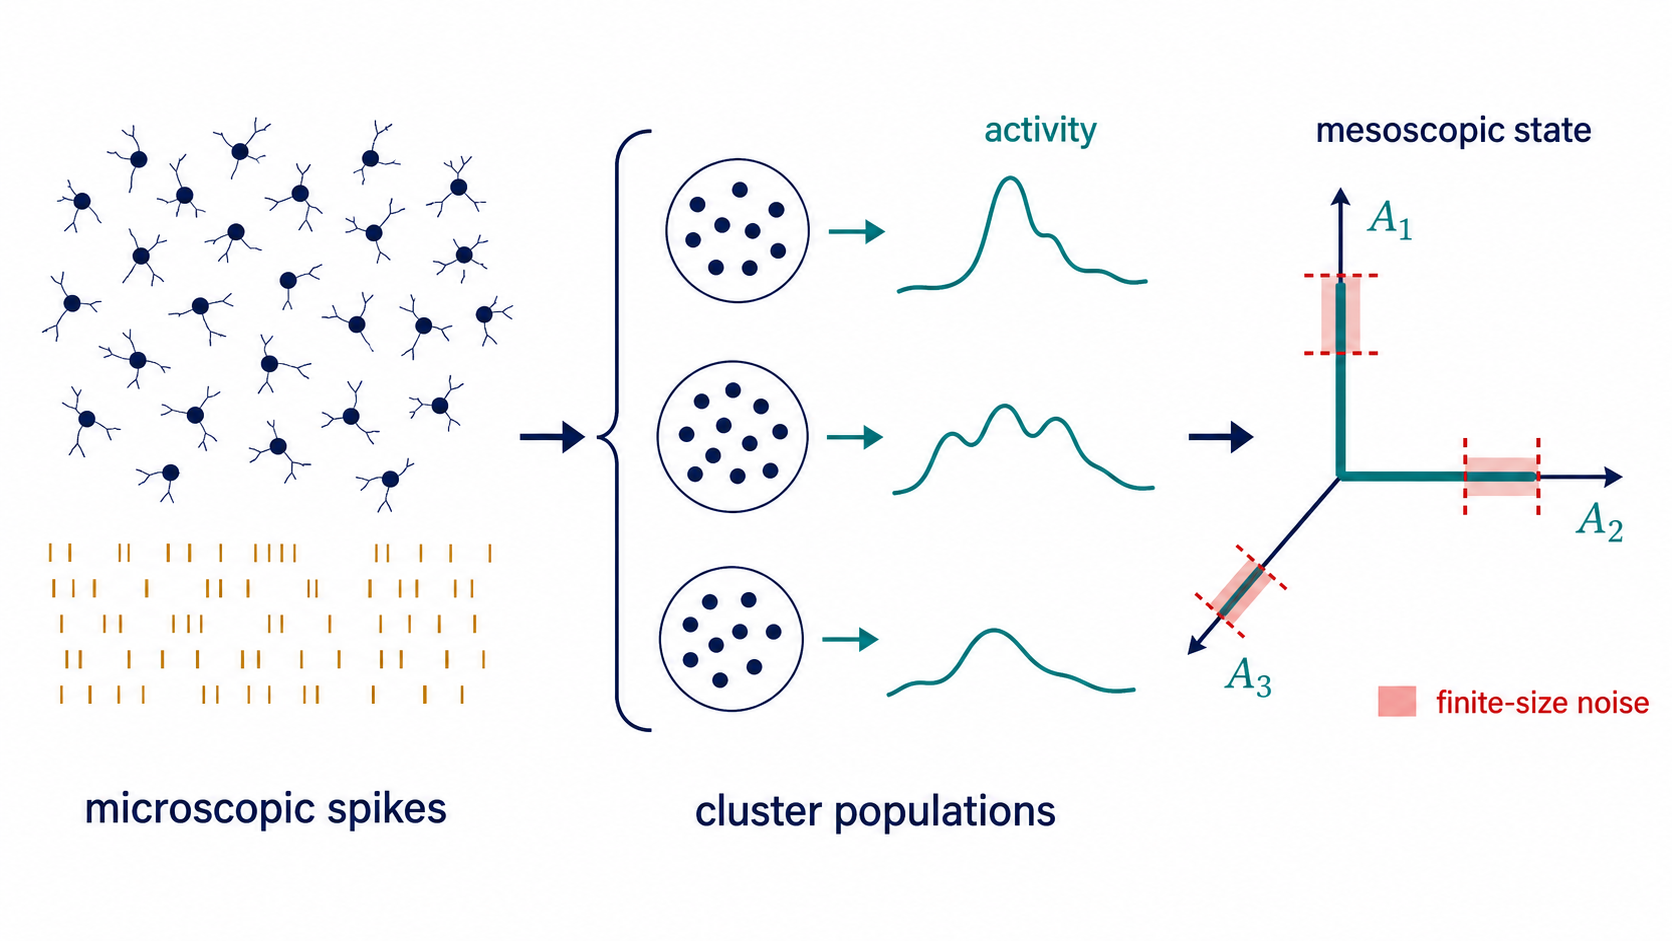
\includegraphics[width=0.95\textwidth]{figures/meso-micro-to-meso-reduction.png}
\caption{The mesoscopic reduction changes the unit of description. Instead of tracking every neuron and spike identity, it groups neurons into cluster populations and follows activity variables such as $A_1$, $A_2$, and $A_3$. Finite-size noise records the residual variability that remains because each population contains finitely many neurons.}
\label{fig:micro-to-meso-reduction}
\end{figure}

% ============================================================
\section{What should a mesoscopic variable represent?}
\label{sec:what-should-mesoscopic-variable-represent}
% ============================================================

A good mesoscopic variable should be tied to both measurement and mechanism. It should answer three questions.

First, what physical or statistical object does it average? For cluster $\alpha$, $A_\alpha$ averages spike trains over neurons. For an E/I-clustered model, we may need two variables per cluster,
%
\begin{equation}
  A_{\alpha E}(t)
  =
  \frac{1}{N_{\alpha E}}\sum_{i\in \alpha E} X_i(t),
  \qquad
  A_{\alpha I}(t)
  =
  \frac{1}{N_{\alpha I}}\sum_{i\in \alpha I} X_i(t).
  \label{eq:ei-cluster-activities}
\end{equation}
%
The first measures excitatory output from cluster $\alpha$; the second measures local inhibitory output. Their difference is not the only relevant quantity, because excitation and inhibition have different synaptic signs, time constants, and effects on gain.

Second, what mechanism changes it? $A_{\alpha E}$ increases when excitatory neurons in cluster $\alpha$ receive enough recurrent excitation to cross threshold. It decreases because of leak, refractoriness, adaptation, synaptic depression, or inhibitory feedback. $A_{\alpha I}$ may follow $A_{\alpha E}$ if inhibitory clusters are paired with excitatory clusters.

Third, what variation is meaningful? Across trials, $A_\alpha(t)$ may fluctuate because the cluster is sometimes in an up-state and sometimes in a down-state. Within one state, the same variable also fluctuates because spike counts are finite. These two sources have different interpretations: state switching is a slow collective event; point-process variability is fast sampling noise.

\begin{aside}[Notation checkpoint]
In these notes, $A_\alpha(t)$ denotes empirical population activity, $R_\alpha(t)$ denotes a filtered or model-predicted population rate, and $\Phi_\alpha$ denotes a transfer function from input to expected activity. Later chapters may specialize $\alpha$ to an excitatory cluster, inhibitory cluster, or unclustered background population.
\end{aside}

% ============================================================
\section{Population rate, population activity, and finite-size noise}
\label{sec:population-rate-activity-finite-size-noise}
% ============================================================

The distinction between rate and activity is essential. The population rate is an expectation. The population activity is what one finite network actually produces.

Let $K_\alpha(t,\Delta t)$ be the number of spikes emitted by cluster $\alpha$ in a time bin $[t,t+\Delta t]$. The empirical activity in that bin is
%
\begin{equation}
  \widehat A_\alpha(t;\Delta t)
  =
  \frac{K_\alpha(t,\Delta t)}{N_\alpha \Delta t}.
  \label{eq:binned-population-activity}
\end{equation}
%
If neurons are conditionally independent Poisson processes with common instantaneous rate $r_\alpha(t)$ during a short bin, then
%
\begin{equation}
  \E[\widehat A_\alpha(t;\Delta t)]
  =
  r_\alpha(t),
  \qquad
  \Var[\widehat A_\alpha(t;\Delta t)]
  =
  \frac{r_\alpha(t)}{N_\alpha \Delta t}.
  \label{eq:finite-size-activity-variance}
\end{equation}
%
The mean is the underlying rate. The variance decreases when the cluster contains more neurons or when the counting window is longer. It increases with the rate because more spikes create more counting variance.

This simple formula explains the square-root scaling used in mesoscopic Langevin equations. The standard deviation is
%
\begin{equation}
  \sqrt{\Var[\widehat A_\alpha]}
  =
  \sqrt{\frac{r_\alpha}{N_\alpha \Delta t}},
  \label{eq:finite-size-standard-deviation}
\end{equation}
%
so fluctuations around the mean shrink like $N_\alpha^{-1/2}$. If cluster size is doubled, intrinsic activity fluctuations are not halved; they are reduced by a factor of $\sqrt{2}$.

Clustered networks complicate this independent-Poisson baseline. Shared input and recurrent coupling introduce correlations:
%
\begin{equation}
  \Var\!\left[\frac{1}{N_\alpha}\sum_{i\in\alpha} K_i\right]
  =
  \frac{1}{N_\alpha^2}
  \left[
    \sum_{i\in\alpha}\Var[K_i]
    +
    \sum_{\substack{i,j\in\alpha\\i\ne j}}\operatorname{Cov}[K_i,K_j]
  \right].
  \label{eq:population-variance-correlations}
\end{equation}
%
The first sum is private spiking noise. The second sum is shared fluctuation. If pairwise covariances remain positive as $N_\alpha$ grows, the population average does not self-average as quickly as independent spikes would predict. This is one reason mesoscopic variables must be checked against microscopic simulations rather than assumed from textbook Poisson scaling.

% ============================================================
\section{When can a cluster be treated as a population?}
\label{sec:when-cluster-treated-population}
% ============================================================

A cluster can be treated as a population when neurons inside it are sufficiently exchangeable for the question being asked. Exchangeability does not mean the neurons are identical. It means that the theory can ignore labels within the cluster and still predict the relevant cluster-level observables.

For an excitatory cluster $\alpha$, the approximation is strongest when:
%
\begin{enumerate}[leftmargin=*]
  \item neurons in the cluster receive statistically similar recurrent input from the same cluster;
  \item heterogeneity in thresholds, degrees, and synaptic weights is small enough to be absorbed into an effective transfer function;
  \item within-cluster correlations are either weak, measurable, or modeled by a corrected noise term;
  \item the target observables are cluster rates, up-state lifetimes, transition probabilities, and autocorrelation times, not precise spike-time motifs.
\end{enumerate}
%
The approximation is weakest when a cluster contains internal substructure that matters dynamically. For example, if a few hub neurons control transitions, replacing the whole cluster by one rate variable can hide the actual switching coordinate. If inhibition is locally paired with excitation, an E-only cluster variable may also be insufficient; the cluster may need both $R_{\alpha E}$ and $R_{\alpha I}$.

The practical test is predictive compression. A mesoscopic cluster variable is appropriate if it predicts the next-time distribution of cluster activity approximately as well as the full microscopic state, after conditioning on the retained variables:
%
\begin{equation}
  \mathbb{P}\!\left(A(t+\Delta t)\mid \text{full microscopic state at }t\right)
  \approx
  \mathbb{P}\!\left(A(t+\Delta t)\mid \vec R(t),\vec Z(t)\right),
  \label{eq:predictive-compression}
\end{equation}
%
where $\vec Z$ denotes additional retained mesoscopic variables such as adaptation, synaptic depression, refractory mass, or filtered input. The left side is exact but high-dimensional. The right side is useful only if the retained state carries the slow information relevant to switching.

% ============================================================
\section{What is lost in the mesoscopic reduction?}
\label{sec:what-is-lost-mesoscopic}
% ============================================================

Mesoscopic reduction deliberately discards microscopic labels. This loses several kinds of information.

It loses exact spike timing. The variable $A_\alpha(t)$ records how much the cluster fired, not which neuron fired first or whether a precise spike sequence occurred. If millisecond-scale synchrony is essential, a one-rate-per-cluster model may be too coarse.

It loses neuron-to-neuron heterogeneity unless that heterogeneity is explicitly represented. Degree distribution, threshold variation, synaptic weight disorder, and spatial structure may all change the effective transfer function. If they are averaged away, the mesoscopic model can fit one parameter regime while failing in another.

It loses quenched disorder at the level of individual connectivity. A finite random connectivity matrix is not exactly equal to its expectation. Some clusters may be accidentally stronger than others. This fixed randomness can bias attractor depths and transition rates across states.

It also loses detailed correlation structure. A population activity variable gives a mean and, with a noise term, perhaps a variance. But microscopic simulations can contain structured correlations across neurons and clusters that require additional variables or colored noise.

These losses are acceptable only if they do not erase the mechanism under study. For the rotation, the dangerous loss is the distinction between deterministic collective instability and finite-size stochastic switching. A mesoscopic model must preserve enough state and noise structure to make that distinction testable.

% ============================================================
\section{What is gained?}
\label{sec:what-is-gained-mesoscopic}
% ============================================================

The gain is that a mesoscopic model turns simulation observations into analyzable objects. Once cluster activity is a state vector $\vec R(t)$, one can compute fixed points, Jacobians, eigenvalues, barriers, switching rates, and finite-size scaling.

For example, suppose a clustered network has a deterministic mesoscopic drift
%
\begin{equation}
  \dot{\vec R} = \vec f(\vec R;\theta),
  \label{eq:deterministic-mesoscopic-drift}
\end{equation}
%
where $\theta$ collects cluster strength, inhibition, external drive, and adaptation parameters. A cluster up-state is a fixed point or metastable region of this drift. Stability is decided by the Jacobian
%
\begin{equation}
  \Jac(\vec R^*) =
  \left[
    \pd{f_\alpha}{R_\beta}(\vec R^*;\theta)
  \right]_{\alpha,\beta}.
  \label{eq:mesoscopic-jacobian}
\end{equation}
%
If all eigenvalues of $\Jac(\vec R^*)$ have negative real part, small perturbations decay and the state is locally stable. If an eigenvalue crosses zero, a saddle-node or pitchfork-like transition can create or destroy a cluster up-state. If a complex pair crosses the imaginary axis, oscillatory or unstable population dynamics can emerge.

Adding finite-size noise gives
%
\begin{equation}
  \dd \vec R
  =
  \vec f(\vec R;\theta)\,\dd t
  +
  \mat G(\vec R;\theta,N)\,\dd \vec W_t,
  \qquad
  \mat G = O(N^{-1/2}),
  \label{eq:mesoscopic-sde-general}
\end{equation}
%
where $\vec W_t$ is a vector of Wiener processes and $\mat G$ sets the amplitude and covariance of population fluctuations. This form makes a concrete prediction: if switching is finite-size driven, increasing cluster size while holding deterministic parameters fixed should lengthen dwell times strongly. If switching persists at comparable strength as $N\to\infty$, finite-size noise is not the whole explanation.

The mesoscopic level therefore supplies the bridge needed for the project:
%
\begin{enumerate}[leftmargin=*]
  \item microscopic simulations show what the network does;
  \item mesoscopic variables identify what collective state is moving;
  \item deterministic analysis explains which states exist and whether they are stable;
  \item finite-size stochastic analysis predicts how often the system switches between them.
\end{enumerate}

\begin{chaptersummary}

\begin{center}
\renewcommand{\arraystretch}{1.55}
\begin{tabularx}{\textwidth}{@{}l X X@{}}
  \toprule
  \textbf{Level} & \textbf{Typical variable} & \textbf{What it explains} \\
  \midrule
  Microscopic &
  $X_i(t)$, $V_i(t)$, synaptic states &
  Exact spike generation and cell-level mechanisms \\
  Macroscopic &
  Global rates $r_E,r_I$ &
  Low-dimensional fixed points and gain, often phenomenological \\
  Mesoscopic &
  Cluster activities $A_\alpha$, filtered rates $R_\alpha$ &
  Population states, finite-size noise, metastable switching \\
  Finite-size scaling &
  $\operatorname{sd}(\widehat A_\alpha)\sim N_\alpha^{-1/2}$ &
  How switching should change with cluster size \\
  Cluster adequacy &
  Predictive compression by $\vec R,\vec Z$ &
  Whether labels inside a cluster can be averaged away \\
  \bottomrule
\end{tabularx}
\end{center}

\end{chaptersummary}

\begin{conceptquestions}
  \item In \cref{eq:microscopic-synaptic-drive}, which terms are microscopic and which could be replaced by population averages?
  \item Why is a deterministic rate model not enough to decide whether switching is caused by finite-size fluctuations?
  \item Derive the scaling $\Var[\widehat A_\alpha]=r_\alpha/(N_\alpha\Delta t)$ for conditionally independent Poisson neurons.
  \item How do positive pairwise correlations change the self-averaging of a population activity variable?
  \item Give one observable that a one-rate-per-cluster model should reproduce and one observable it is allowed to discard.
  \item What experiment or simulation would you run to test whether a cluster-level variable is a good predictive compression of the microscopic state?
  \item If switching dwell times do not increase when cluster size is increased, what does that imply about a finite-size switching hypothesis?
\end{conceptquestions}
